
\documentclass[final]{cvpr}

\usepackage{times}
\usepackage{epsfig}
\usepackage{graphicx}
\usepackage{amsmath}
\usepackage{amssymb}

\usepackage{enumitem}
\usepackage{booktabs}

\usepackage{pgfplots} \usepackage{pgfplotstable} \pgfplotsset{compat=newest} \usetikzlibrary{plotmarks} \usetikzlibrary{colorbrewer} 

\usepackage{xspace}

\usepackage{algorithm}
\usepackage{algpseudocode}
\usepackage{multirow}
\usepackage{tabularx}
\usepackage{wrapfig}
\usepackage{stfloats}  

\makeatletter
\DeclareRobustCommand\onedot{\futurelet\@let@token\@onedot}
\def\@onedot{\ifx\@let@token.\else.\null\fi\xspace}

\usepackage[pagebackref=true,breaklinks=true,colorlinks,bookmarks=false]{hyperref}

\def\eg{\emph{e.g}\onedot} \def\Eg{\emph{E.g}\onedot}
\def\ie{\emph{i.e}\onedot} \def\Ie{\emph{I.e}\onedot}
\def\cf{\emph{cf}\onedot} \def\Cf{\emph{Cf}\onedot}
\def\etc{\emph{etc}\onedot} \def\vs{\emph{vs}\onedot}
\def\wrt{w.r.t\onedot} \def\dof{d.o.f\onedot}
\def\etal{\emph{et al}\onedot}


\newcommand{\algoref}[1]{Alg\onedot~\ref{#1}}

\usepackage{pifont}
\newcommand{\cmark}{\ding{51}}
\newcommand{\xmark}{\ding{55}}



\def\cvprPaperID{1280} \def\confYear{CVPR 2021}


\begin{document}

\title{Scaling Wide Residual Networks for Panoptic Segmentation}

\author{Liang-Chieh Chen\textsuperscript{1}~~~~~~Huiyu Wang\textsuperscript{2}\thanks{Work done while an intern at Google.}~~~~~~Siyuan Qiao\textsuperscript{2}\footnotemark[1]\\
\textsuperscript{1}Google Research\\\textsuperscript{2}Johns Hopkins University\\
}


\maketitle

\begin{abstract}
The Wide Residual Networks (Wide-ResNets), a shallow but wide model variant of the Residual Networks (ResNets) by stacking a small number of residual blocks with large channel sizes, have demonstrated outstanding performance on multiple dense prediction tasks. However, since proposed, the Wide-ResNet architecture has barely evolved over the years. In this work, we revisit its architecture design for the recent challenging panoptic segmentation task, which aims to unify semantic segmentation and instance segmentation. A baseline model is obtained by incorporating the simple and effective Squeeze-and-Excitation and Switchable Atrous Convolution to the Wide-ResNets. Its network capacity is further scaled up or down by adjusting the width (\ie, channel size) and depth (\ie, number of layers), resulting in a family of SWideRNets (short for Scaling Wide Residual Networks). We demonstrate that such a simple scaling scheme, coupled with grid search, identifies several SWideRNets that significantly advance state-of-the-art performance on panoptic segmentation datasets in both the fast model regime and strong model regime.
\end{abstract}
 \section{Introduction}
\label{sec:intro}


\begin{figure}
    \hspace{-4mm}
    \begin{tabular} {c}
    \vspace{-2mm}
    \resizebox{\linewidth}{!}{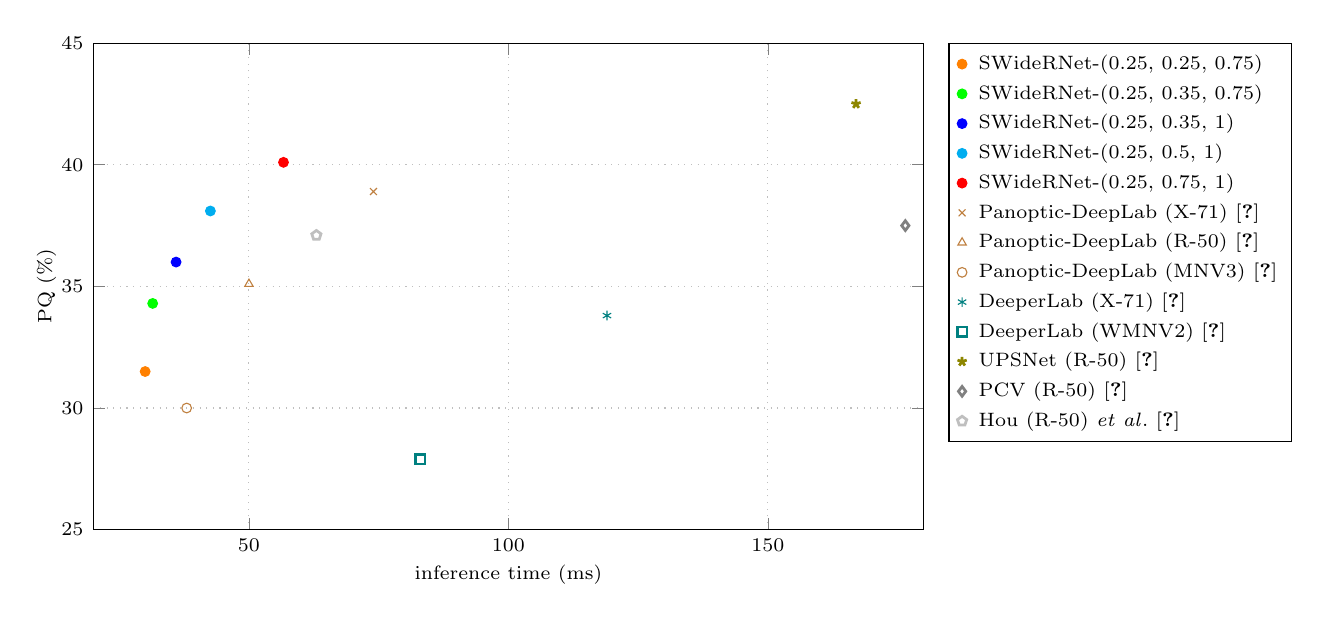
\begin{tikzpicture}[/pgfplots/width=1\linewidth, /pgfplots/height=0.64\linewidth, /pgfplots/legend pos=south east]
    \begin{axis}[
        ymin=25,ymax=45,xmin=20,xmax=180,
        xlabel=inference time (ms),
        ylabel=PQ (\%),
		font=\scriptsize,
        grid=both,
		grid style=dotted,
        legend columns=1,
        xlabel shift={-2pt},
        ylabel shift={-5pt},
xtick={0,50,...,300},
ytick={0,5,...,60},
        legend pos= outer north east,
        legend cell align={left},
        legend style={font=\scriptsize},
        ]

        
	    \addplot[orange,mark=*,only marks,mark size=1.75] coordinates{(30, 31.5)};
        \addlegendentry{\hphantom{i}SWideRNet-(0.25, 0.25, 0.75)}
        
        \addplot[green,mark=*,only marks,mark size=1.75] coordinates{(31.45, 34.3)};
        \addlegendentry{\hphantom{i}SWideRNet-(0.25, 0.35, 0.75)}
        
        \addplot[blue,mark=*,only marks,mark size=1.75] coordinates{(35.96, 36)};
        \addlegendentry{\hphantom{i}SWideRNet-(0.25, 0.35, 1)}
        
        \addplot[cyan,mark=*,only marks,mark size=1.75] coordinates{(42.57, 38.1)};
        \addlegendentry{\hphantom{i}SWideRNet-(0.25, 0.5, 1)}
        
        \addplot[red,mark=*,only marks,mark size=1.75] coordinates{(56.66, 40.1)};
        \addlegendentry{\hphantom{i}SWideRNet-(0.25, 0.75, 1)}
        
	    \addplot[brown,mark=x,only marks,mark size=1.75] coordinates{(74, 38.9)};
        \addlegendentry{\hphantom{i}Panoptic-DeepLab (X-71) \cite{cheng2019panoptic}}
    
        \addplot[brown,mark=triangle,only marks,mark size=1.75] coordinates{(50, 35.1)};
        \addlegendentry{\hphantom{i}Panoptic-DeepLab (R-50) \cite{cheng2019panoptic}}

        \addplot[brown,mark=o,only marks,mark size=1.75] coordinates{(38, 30.0)};
        \addlegendentry{\hphantom{i}Panoptic-DeepLab (MNV3) \cite{cheng2019panoptic}}

        \addplot[teal,mark=asterisk,only marks,mark size=1.75] coordinates{(119, 33.8)};
        \addlegendentry{\hphantom{i}DeeperLab (X-71) \cite{yang2019deeperlab}}
       
        \addplot[teal,mark=square,only marks,line width=1, mark size=1.75] coordinates{(83, 27.9)};
        \addlegendentry{\hphantom{i}DeeperLab (WMNV2) \cite{yang2019deeperlab}}

        \addplot[olive,mark=star, mark size=1.75,only marks, line width=1] coordinates{(167, 42.5)};
        \addlegendentry{\hphantom{i}UPSNet (R-50) \cite{xiong2019upsnet}}
        
        \addplot[gray,mark=diamond, mark size=1.75,only marks, line width=1] coordinates{(176.5, 37.5)};
        \addlegendentry{\hphantom{i}PCV (R-50) \cite{Wang_2020_CVPR}}
        
        \addplot[lightgray,mark=pentagon, mark size=1.75,only marks, line width=1] coordinates{(63, 37.1)};
        \addlegendentry{\hphantom{i}Hou (R-50) \etal \cite{hou2020real}}
        
    \end{axis}
\end{tikzpicture}}
  \\
    {\scriptsize (a) PQ \vs inference time (ms) on COCO val set.} \\
    \vspace{-2mm}
    \resizebox{\linewidth}{!}{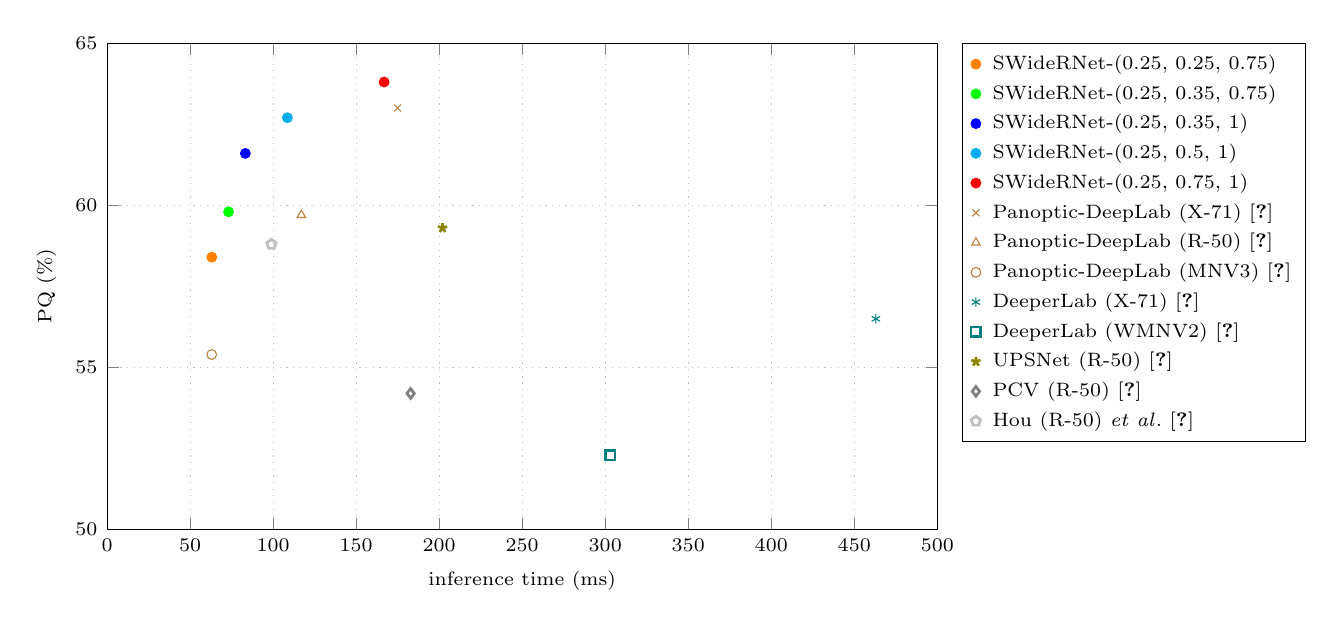
\begin{tikzpicture}[/pgfplots/width=1\linewidth, /pgfplots/height=0.64\linewidth, /pgfplots/legend pos=south east]
    \begin{axis}[
        ymin=50,ymax=65,xmin=0,xmax=500,
        xlabel=inference time (ms),
        ylabel=PQ (\%),
		font=\scriptsize,
        grid=both,
		grid style=dotted,
        legend columns=1,
xtick={0,50,...,500},
ytick={0,5,...,70},
        legend pos= outer north east,
        legend cell align={left}
        ]

        \addplot[orange,mark=*,only marks,mark size=1.75] coordinates{(63.05, 58.4)};
        \addlegendentry{\hphantom{i}SWideRNet-(0.25, 0.25, 0.75)}
        
        \addplot[green,mark=*,only marks,mark size=1.75] coordinates{(73.14, 59.8)};
        \addlegendentry{\hphantom{i}SWideRNet-(0.25, 0.35, 0.75)}
        
        \addplot[blue,mark=*,only marks,mark size=1.75] coordinates{(83.25, 61.6)};
        \addlegendentry{\hphantom{i}SWideRNet-(0.25, 0.35, 1)}
        
        \addplot[cyan,mark=*,only marks,mark size=1.75] coordinates{(108.58, 62.7)};
        \addlegendentry{\hphantom{i}SWideRNet-(0.25, 0.5, 1)}
        
        \addplot[red,mark=*,only marks,mark size=1.75] coordinates{(166.83, 63.8)};
        \addlegendentry{\hphantom{i}SWideRNet-(0.25, 0.75, 1)}
        
	    \addplot[brown,mark=x,only marks,mark size=1.75] coordinates{(175, 63)};
        \addlegendentry{\hphantom{i}Panoptic-DeepLab (X-71) \cite{cheng2019panoptic}}
        
        \addplot[brown,mark=triangle,only marks,mark size=1.75] coordinates{(117, 59.7)};
        \addlegendentry{\hphantom{i}Panoptic-DeepLab (R-50) \cite{cheng2019panoptic}}

        \addplot[brown,mark=o,only marks,mark size=1.75] coordinates{(63, 55.4)};
        \addlegendentry{\hphantom{i}Panoptic-DeepLab (MNV3) \cite{cheng2019panoptic}}

        \addplot[teal,mark=asterisk,only marks,mark size=1.75] coordinates{(463, 56.5)};
        \addlegendentry{\hphantom{i}DeeperLab (X-71) \cite{yang2019deeperlab}}
       
        \addplot[teal,mark=square,only marks,line width=1, mark size=1.75] coordinates{(303, 52.3)};
        \addlegendentry{\hphantom{i}DeeperLab (WMNV2) \cite{yang2019deeperlab}}

        \addplot[olive,mark=star, mark size=1.75,only marks, line width=1] coordinates{(202, 59.3)};
        \addlegendentry{\hphantom{i}UPSNet (R-50) \cite{xiong2019upsnet}}
        
        \addplot[gray,mark=diamond, mark size=1.75,only marks, line width=1] coordinates{(182.8, 54.2)};
        \addlegendentry{\hphantom{i}PCV (R-50) \cite{Wang_2020_CVPR}}
        
        \addplot[lightgray,mark=pentagon, mark size=1.75,only marks, line width=1] coordinates{(99, 58.8)};
        \addlegendentry{\hphantom{i}Hou (R-50) \etal \cite{hou2020real}}
    \end{axis}
\end{tikzpicture}}
  \\
    {\scriptsize (b) PQ \vs inference time (ms) on Cityscapes Vistas val set} \\
    \vspace{-2mm}
    \end{tabular}
    \caption{PQ \vs GPU inference time. Our fast SWideRNet model variants, deployed as the network backbone in  Panoptic-DeepLab~\cite{cheng2019panoptic}, significantly improve the speed-accuracy trade-off.
    }
    \vspace{-2mm}
    \label{fig:pq_vs_second}
\end{figure}

Computer vision systems have achieved remarkable performance across a wide range of image recognition tasks, including image classification~\cite{krizhevsky2012imagenet,simonyan2014very}, object detection~\cite{girshick2014rich,ren2015faster}, and dense prediction~\cite{long2015fully,deeplabv12015}, thanks to the recent advances in  learning algorithms~\cite{goodfellow2016deep} (\eg, better optimizer~\cite{kingma2015adam}, normalization techniques~\cite{ioffe2015batch,salimans2016weight,wu2018group,qiao2019weight}, and scalable training systems~\cite{tensorflow-osdi2016,goyal2017accurate,peng2018megdet}). The improvement of neural network architectures especially plays an important role, as manifested on public benchmarks~\cite{everingham2010pascal,lin2014microsoft,ILSVRC15}. 

Gaining in popularity for its simplicity and effectiveness, Residual Networks (ResNets)~\cite{he2016deep} have been the building blocks of many modern neural network architectures~\cite{wrn2016wide,xie2017aggregated,hu2018squeeze,wu2019wider,li2019selective,gao2019res2net,radosavovic2020designing,zhang2020resnest}. Specifically, the Wide-ResNets~\cite{wrn2016wide} adopt the `shallow but wide' architecture design (\ie, fewer layers but with large channels) and show superior performance over the `deep but thin' architectures (\ie, more layers but with small channels). Along the same direction, the Wide-ResNet-38 (WR-38)~\cite{wu2019wider}, a sophisticated human-designed wide residual network, is one of the top-performing network backbones on many dense prediction benchmarks~\cite{cordts2016cityscapes,neuhold2017mapillary}.
However, since proposed in 2016, the architecture of WR-38 has barely evolved over the years.
Recently, a simple modification of WR-38, by altering the last two residual blocks, leads to a slightly better and faster architecture WR-41~\cite{chen2020naive}, when deployed as the network backbone in  Panoptic-DeepLab~\cite{cheng2019panoptic} framework. The resulting model has shown state-of-the-art performance for panoptic  segmentation~\cite{kirillov2018panoptic}, which is a challenging dense prediction task with the goal to unify semantic segmentation~\cite{he2004multiscale} and instance segmentation~\cite{hariharan2014simultaneous}. 

In this work, we ask if we may revisit the architecture design of wide residual networks to further boost the panoptic segmentation performance and even improve the model inference speed.
In particular, a baseline model is obtained by equipping the WR-41~\cite{chen2020naive} with the simple and effective modules, Squeeze-and-Excitation (SE)~\cite{hu2018squeeze} and Switchable Atrous Convoloution (SAC)~\cite{qiao2020detectors}. Similar to~\cite{wrn2016wide,howard2017mobilenets,tan2019efficientnet}, its network capacity could be further adjusted by three scaling factors , where  controls the channel size of the first two stages of a network backbone, while  and  adjust the network width (\ie, channel size) and depth (\ie, number of layers) of the remaining stages, respectively. The resulting model SWideRNet- (short for {\bf S}caling {\bf W}ide {\bf R}esidual Network with scaling factors ) is deployed as the network backbone in Panoptic-DeepLab~\cite{cheng2019panoptic} framework.

The SWideRNet- defines a large number of backbone architectures, targeting for different applications. The search space for those three scaling factors is discretized, allowing us to employ the simple and effective grid search method. Two model regimes are considered in this work, where the first one contains fast model variants and the other contains strong architectures. As a result, our main contribution lies in empirically identifying several fast SWideRNet backbones that attain state-of-the-art speed-accuracy trade-off, as well as several strong SWideRNet backbones that further push the envelope of panoptic segmentation benchmarks. As shown in \figref{fig:pq_vs_second}, our fast SWideRNets attain a better speed-accuracy trade-off than prior state-of-the-art models, showing at least 3\% PQ better than the MobileNetv3~\cite{howard2019searching} backbone at a similar speed. Interestingly, the found fast SWideRNets all share the same scaling factor , indicating that the first two stages of Wide-ResNets are the speed bottleneck.
Finally, for the strong model regime, we found that going deeper (\ie, only increasing ) is the most efficient strategy to scale up the network capacity, suggesting that the Wide-ResNets may be already sufficiently `wide'. 
Our strong SWideRNet model variants consistently outperform prior {\it bottom-up} state-of-the-art Axial-DeepLab~\cite{wang2020axial} on three datasets.
Additionally, our {\it single} model outperforms ensemble models on Mapillary Vistas and ADE20K.
 \section{Related Works}
\label{sec:related}

{\bf Convolutional Neural Networks:} 
Convolutional Neural Networks (CNNs)~\cite{lecun1998gradient} deployed in a fully convolutional manner (FCNs~\cite{sermanet2014overfeat,long2015fully}) have achieved remarkable performance on dense prediction tasks. The improvement of neural network design is one of the main driving forces for state-of-the-art systems, from AlexNet~\cite{krizhevsky2012imagenet}, VGG~\cite{simonyan2014very}, Inception~\cite{ioffe2015batch,szegedy2016rethinking,szegedy2017inception}, ResNet~\cite{he2016deep,he2016identity} to more recent architectures, such as  DenseNet~\cite{huang2017densely}, Xception~\cite{chollet2017xception, dai2017coco}, and EfficientNet~\cite{tan2019efficientnet}. Due to the simple yet effective design of residual networks~\cite{he2016deep}, there are many modern neural networks that build on top of it, including Wide-ResNet~\cite{wrn2016wide,wu2019wider}, ResNeXt~\cite{xie2017aggregated}, 
SENet~\cite{hu2018squeeze}, SKNet~\cite{li2019selective}
Res2Net~\cite{gao2019res2net}, RegNet~\cite{radosavovic2020designing}, and ResNeSt~\cite{zhang2020resnest}. 

\begin{figure*}[!t]
    \centering
    \scalebox{0.8}{
    \begin{tabular}{c | c}
    \includegraphics[height=0.46\textwidth]{figures/module/se.pdf} &
    \includegraphics[height=0.46\textwidth]{figures/module/sac.pdf} \\
    (a) Squeeze-and-Excitation &
    (b) Switchable Atrous Convolution \\
    \end{tabular}
    }
    \caption{Illustration of our employment of (a) Squeeze-and-Excitation (SE) module and (b) Swithcable Atrous Convolution (SAC).}
    \label{fig:modules}
\end{figure*}

{\bf Scaling CNNs:} The capacity of Convolutional Neural Networks (CNNs) could be scaled up by stacking more convolutional layers or increasing the channels. ResNet~\cite{he2016deep} is the first work that successfully stacks over 1000 convolutional layers for small-resolution images, while PSPNet~\cite{zhao2017pyramid} employs ResNet with 269 layers, and shows outstanding semantic segmentation results. MobileNets~\cite{howard2017mobilenets,sandler2018mobilenetv2,howard2019searching} and ShuffleNets~\cite{ma2018shufflenet,ma2018shufflenet} introduce a universal scaling factor to adjust network channels. Wide-ResNet~\cite{wrn2016wide,wu2019wider}, GPipe~\cite{gpipe18}, and BiT~\cite{kolesnikov2020big} explore scaling up both layers and channels for image classification. Auto-DeepLab~\cite{liu2019auto} increases the channels of a base network for better semantic segmentation performance. More recently, EfficientNet~\cite{tan2019efficientnet} and EfficientDet~\cite{tan2020efficientdet} adopt a compound factor to effectively and simultaneously scaling up layers, channels, and input resolutions for image classification and object detection, respectively. Our model follows the same direction by scaling the architecture of Wide-ResNet~\cite{wrn2016wide,wu2019wider}, specifically targeting for panoptic segmentation~\cite{kirillov2018panoptic}.

{\bf Panoptic Segmentation:} State-of-the-art panoptic segmentation systems could be roughly categorized into top-down (or proposal-based) and bottom-up (or box-free) approaches. Top-down approaches~\cite{kirillov2019panoptic,porzi2019seamless,li2018learning,li2018attention,liu2019e2e,xiong2019upsnet,li2020unifying,Chen_2020_CVPR,Lazarow_2020_CVPR,wu2020bidirectional,wu2020auto} typically pair Mask R-CNN~\cite{he2017mask} with a light-weight `stuff` segmentation branch, while bottom-up approaches~\cite{yang2019deeperlab,gao2019ssap,Wang_2020_CVPR,cheng2019panoptic,wang2020axial} group `thing` pixels from semantic segmentation predictions. Recently, Panoptic-DeepLab~\cite{cheng2019panoptic}, a simple yet effective bottom-up system for panoptic segmentation, employs DeepLab semantic segmentation outputs~\cite{chen2018deeplabv2,deeplabv3plus2018} coupled with a class-agnostic instance segmentation branch involving a simple instance center regression~\cite{kendall2018multi,uhrig2018box2pix,neven2019instance}. Panoptic-DeepLab~\cite{cheng2019panopticworkshop} has achieved state-of-the-art results on several benchmarks, and our method builds on top of it.
 \section{Methods}
\label{sec:methods}
In this section, we describe how to effectively scale the capacity of our baseline model, obtained by incorporating to Wide-ResNet-41 (WR-41)~\cite{wrn2016wide,wu2019wider,chen2020naive} the simple yet effective Squeeze-and-Excitation~\cite{hu2018squeeze} and Switchable Atrous Convolution~\cite{qiao2020detectors} modules. The resulting network family with different scaling factors is then explored for both fast model regime and strong model regime.

\subsection{The SWideRNet family}
{\bf Baseline model:} The Wide Residual Networks~\cite{wrn2016wide,wu2019wider} have demonstrated outstanding performance on image classification~\cite{ILSVRC15}, object detection~\cite{lin2014microsoft}, and semantic segmentation~\cite{everingham2010pascal}. Specifically, the Wide-ResNet-38 (WR-38)~\cite{wu2019wider}, refined by several human-crafted networks with extensive experiments, has been the {\it de facto} network backbone for semantic segmentation~\cite{neuhold2017mapillary,rota2018place,zhu2019improving,takikawa2019gated,li2020improving}, and instance segmentation~\cite{liang2019polytransform,homayounfar2020levelset} on Cityscapes leader-board~\cite{cordts2016cityscapes}. Recently, Chen~\etal~\cite{chen2020naive} attain state-of-the-art panoptic segmentation performance~\cite{kirillov2018panoptic} on Cityscapes~\cite{cordts2016cityscapes} by employing the Wide-ResNet-41 (WR-41), which improves both accuracy and speed over the WR-38~\cite{wu2019wider} (when deploying in the Panoptic-DeepLab~\cite{cheng2019panoptic} framework) by (1) removing the last residual block, and (2) repeating the second last residual block two more times.

Building on top of WR-41, we further incorporate the simplified Squeeze-and-Excitation (SE) module~\cite{hu2018squeeze,lee2020centermask} (where only one fully connected layer is used), and the Switchable Atrous Convolution (SAC)~\cite{qiao2020detectors}, forming our baseline model. In  \figref{fig:modules}, we visualize the simplified SE module and SAC operation. To be concrete, the channel attention map  in the SE module is computed as follows.

where  is the globally average-pooled input feature map, and  are the weights of a fully connected layer. Following~\cite{howard2019searching}, we employ the hard sigmoid function~\cite{binaryconnect}: .

\newcommand{\blocka}[2]{\multirow{3}{*}{-.1em] \text{33, #1} \end{array}\right]\times\times\times\left[\begin{array}{c}\text{11, #1}\-.1em] \text{11, #3}\end{array}\right]\timesw_1w_2\ell\times\times\times\times\times w_1\times\times\times w_1\times\times\times\times w_2\ell\times\times\times w_2\ell\times\times\times w_2\ell\times\times\times w_2\times w_2\times w_2\ell\times\timesw_1w_2\ell\mathbf{y}=\text{\bf Conv}(\mathbf{x}, \mathbf{w}, r)\mathbf{w}r\mathbf{x}\mathbf{y}\mathbf{S}r\mathbf{w}\mathbf{S}5\times51\times1(w_1, w_2, \ell)w_1w_2\ell(w_1, w_2, \ell)(w_1, w_2, \ell)7 + 33 \times \ell(w_1, w_2, \ell)(w_1, w_2, \ell)(w_1, w_2, \ell)\boldsymbol{S}_{fast}(w_1, w_2, \ell)\boldsymbol{S}_{strong}1024\times7684000\times60000.0001641\times6411025\times10251025\times20491025\times2049641\times641\{0.5, 0.75, 1, 1.25, 1.5\}\{0.5, 0.75, 1, 1.25, 1.5, 1.75, 2\}\{1, 2, 4\}w_1=0.25\ellw_2w_2\ell641\times6411025\times1025\dagger1025\times1025\dagger\dagger\dagger:1025\times10251025\times20491025\times20491025\times20491025\times20491025\times2049641\times641641\times641800\times1333800\times1333641\times641641\times641641\times6411025\times1025800\times1333641\times641641\times641641\times641641\times641641\times6411024\times20481025\times20491025\times20491024\times20481024\times20481025\times20491025\times20491025\times20491025\times20491025\times20491025\times20491025\times20491025\times2049\text{PQ}^{\text{Th}}\text{PQ}^{\text{St}}\dagger\dagger\dagger(w_1, w_2, \ell)$, a family of neural networks by scaling the width (\ie, channel size) and depth (\ie, number of layers) of Wide Residual Networks. Two search spaces are explored, where the first one contains fast model variants, and the other one contains strong architectures. Discretizing the search space allows us to employ the simple but effective grid search. As a result, we empirically identify several fast SWideRNets that attain outstanding performance in terms of speed-accuracy trade-off, and several strong SWideRNets that further advance sate-of-the-art results on several public benchmarks. 

{\bf Acknowledgments }
We would like to thank the discussions with Yukun Zhu and Maxwell Collins, and the support from Google Mobile Vision team.
 

{\small
\bibliographystyle{ieee_fullname}
\bibliography{refs}
}



\end{document}
